\documentclass[10pt]{beamer}

\usepackage[english]{babel}
\usepackage[utf8]{inputenc}
\usepackage{lmodern}
\usepackage{listings}
\usepackage{caption}
\usepackage{subcaption}

\captionsetup[lstlisting]{ margin=0pt }

\definecolor{lgray}{gray}{0.96}
\definecolor{lbcolor}{rgb}{0.9,0.9,0.9}
\lstset{
    framesep=2pt,
    basicstyle=\ttfamily\scriptsize,
    breaklines=true,
    breakatwhitespace=true,
    aboveskip={0.75\baselineskip},
    columns=fixed,
    showstringspaces=false,
    breaklines=true,
    frame=single,
    rulecolor=\color{lgray},
    showtabs=false,
    showspaces=false,
    showstringspaces=false,
    backgroundcolor=\color{lgray},
    identifierstyle=\ttfamily,
    keywordstyle=\color[rgb]{0,0,1},
    commentstyle=\color[rgb]{0.0,0.26,0.15},
    stringstyle=\color[rgb]{0.627,0.126,0.941}
}

\setbeamersize{text margin left=5mm,text margin right=5mm}


\usetheme{AGH}
\title{Update and upgrade of the GGSS system for ATLAS TRT detector}
\author{\normalsize{Arkadiusz Kasprzak \newline \and 
    Jarosław Cierpich \newline \newline \and 
    Supervisor: Bartosz Mindur}}
\date{}

\begin{document}

\titleframe[en]

\begin{frame}
\frametitle{Agenda}
\tableofcontents
\end{frame}


\section {A brief introduction to GGSS}


\begin{frame}
\frametitle{Introduction to GGSS}
\begin{itemize}
\item Gas Gain Stabilization System (GGSS) is a project integrated with ATLAS Detector Control System (DCS).
\item It helps to ensure proper operation of the TRT (Transition Radiation Tracker) detector, which is a part of the ATLAS detector at CERN.
\item GGSS consists of hardware and software layers.
\item Today we will focus mainly on the software layer.
\item Most of the codebase is written using C++. There is also some Python and Bash code. 
\end{itemize}
\end{frame}

\begin{frame}
\frametitle{GGSS software}
\begin{figure}
    \centering
    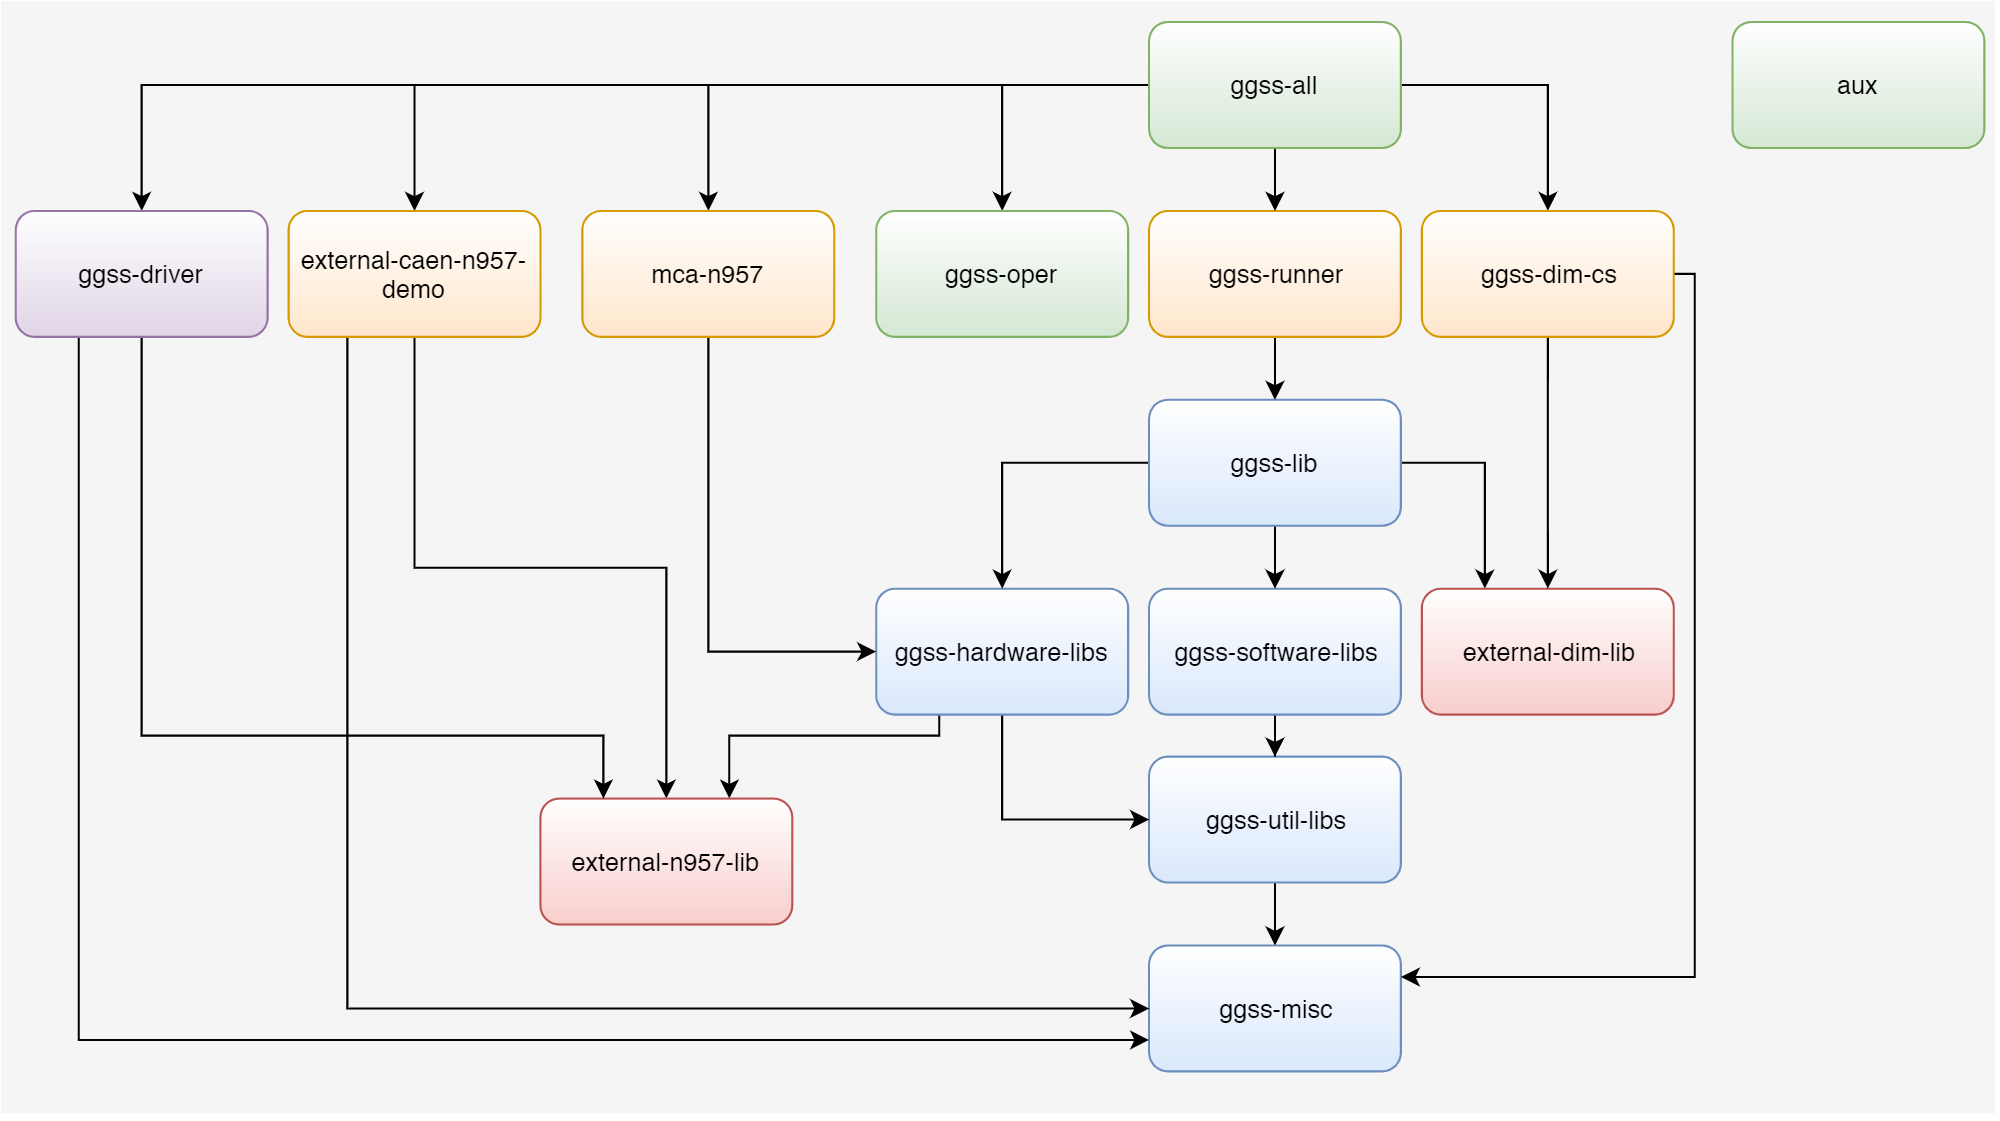
\includegraphics[width=0.87\textwidth]{resources/ggss_software_arch.png}
    \caption{Software components of the GGSS project and their dependencies.}
\end{figure}
\end{frame}


\section {Tasks and constraints}


\begin{frame}
\frametitle{Tasks}
\begin{itemize}
    \item C++ codebase refactoring: \begin{itemize}
        \item migration to C++11/14 (range-for loops, uniform initialization etc)
        \item removing old, unused code 
        \item adding more comprehensive documentation
        \item introducing TDD (Test Driven Development)
    \end{itemize}
    \item CMake files refactoring
    \item creating tools for versioning and Git submodule handling
    \item creating Python library and apps for hardware testing (in progress)
\end{itemize}
\end{frame}

\begin{frame}
\frametitle{Understanding the constraints}
\begin{itemize}
\item The user must be able to build the project using the CERN infractructure
\item Code refactoring had to be performed with this constraints in mind.
\item Only old version of CMake (2.8) and GCC (C++11/14, but no 17/20) available.
\end{itemize}
\end{frame}


\section {Overview of changes}


\begin{frame}[fragile]
\frametitle{Migration to C++11/14}
Example of migration to C++11/14 - replacing iterator loop with range-for one. Below You can see the old code.
\begin{lstlisting}[language=c++, caption={Example of old C++ code (before refactoring).}]
for ( XMLTag::NestedTags::const_iterator j = tag.getNestedTags().begin()
            ; j != tag.getNestedTags().end()
            ; j++
        )
{
    if((j->second->getName() == tagName)
        &&(j->second->getAttributeValue("id") == idValue))
        return j->second;
    else
        m_findTagById(*(j->second), tagName, idValue);		
} // endfor
\end{lstlisting}
\end{frame}


\begin{frame}[fragile]
\frametitle{Migration to C++11/14}
\begin{lstlisting}[language=c++, caption={Example of new C++ code (after refactoring).}]
const XMLTag::NestedTags& nestedTags = startingTag.getNestedTags();
for(const auto& nestedTag: nestedTags)
{
    if((nestedTag.second->getName() == tagName) && (nestedTag.second->getAttributeValue("id") == idValue))
    {
        return nestedTag.second;
    }
}
\end{lstlisting}
\begin{itemize}
    \item using range-for loop increases readability of the code
    \item \lstinline[basicstyle=\ttfamily\normalsize]{else} clause has been removed - result of the recursive function call was never used
    \item no need to use the \lstinline[basicstyle=\ttfamily\normalsize]{*} operator
    \item \lstinline[basicstyle=\ttfamily\normalsize]{nestedTag} is a better name than \lstinline[basicstyle=\ttfamily\normalsize]{j}
\end{itemize}
\end{frame}


\begin{frame}[fragile]
\frametitle{Removing old, unused code}
\begin{itemize}
\item The project contained a lot of code (functions/methods) that were never used.
\item Some of them could even be harmful if used.
\item Below example shows two methods that have been removed (why?) from \lstinline[basicstyle=\ttfamily\normalsize]{QueueLimited} class (a queue with size limit).
\end{itemize}
\begin{lstlisting}[language=c++, caption={Example of removed code.}]
// return the whole queue
const std::deque<T>& getQueue () const {
    return c;
}

// return the whole queue
std::deque<T>& getQueue () {
    return c;
}
\end{lstlisting}
\end{frame}


\begin{frame}[fragile]
\frametitle{Introducing Test Driven Development}
\begin{itemize}
\item For unit tests, we are using \lstinline[basicstyle=\ttfamily\normalsize]{Boost.Test}, because it is simple and available when using CERN infrastructure.
\item Component are tested during refactoring, we make sure that our changes do not introduce any new bugs.
\item Each component can be tested separately.
\end{itemize}
\begin{lstlisting}[language=c++, caption={Unit test example}]
/**
 * \brief Checks if proper exception is thrown when performing pop() 
 *        operation on empty container.
 */
BOOST_AUTO_TEST_CASE(
    testIfExceptionIsThrownWhenTryingToPopFromEmptyContainer)
{
    QueueLimited<int> queue{};
    BOOST_CHECK_THROW(
        queue.pop(), 
        QueueLimited<int>::ReadEmptyQueueException);
}   
\end{lstlisting}
\end{frame}

\begin{frame}[fragile]
\frametitle{Continous Integration}
\begin{itemize}
\item Practice widely used during modern software development.
\item Developers integrate code into repository frequently.
\item Each code contribution is automatically built and tested.
\item This allows for quick error detection.
\item We use GitLab CI/CD for building and testing the project.
\end{itemize}
\begin{figure}
\centering
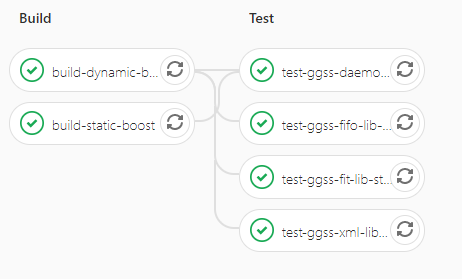
\includegraphics[width=0.5\textwidth]{resources/pipeline_example.png}
\caption{Example of CI pipeline used in the project.}
\end{figure}
\end{frame}


\begin{frame}[fragile]
\frametitle{CMake files refactoring}
\begin{itemize}
\item GGSS uses CMake for managing the build process of the software.
\item CMake is platform and compiler independent.
\item CMake files have been slightly refactored to improve readability by using macros and functions.
\end{itemize}
\begin{lstlisting}[language=c++, caption={Old version of CMake used for building \emph{thread-lib}}]
set(target_name "thread")
if(NOT TARGET ${target_name})
    set(CMAKE_MODULE_PATH "${GGSS_MISC_PATH}")
    include(BuildLibrary)
    include(FindLibraryBoost)
    include(SetupDoxygen)
    include(SetupTests)

    # notice the need to set some variables before including the file
    set(dependency_prefix "${CMAKE_CURRENT_SOURCE_DIR}/..")
    set(dependencies "handle" "log")
    include(BuildDependencies)
endif() 
\end{lstlisting}
\end{frame}


\begin{frame}[fragile]
\frametitle{CMake files refactoring}
\begin{itemize}
\item Instead of including the CMake template files (which just pastes the code), we invoke \lstinline[basicstyle=\ttfamily\normalsize]{ggss_build_library} with named parameters.
\item Unit tests and Doxygen support has been moved to \lstinline[basicstyle=\ttfamily\normalsize]{ggss_build_library} macro, because every library in the project uses them.
\end{itemize}
\begin{lstlisting}[language=c++, caption={New version of CMake used for building \emph{thread-lib}}]
set(CMAKE_MODULE_PATH "${GGSS_MISC_PATH}")
include(BuildLibrary)

ggss_build_library(
    TARGET_NAME "thread"
    DEPENDENCY_PREFIX "${CMAKE_CURRENT_SOURCE_DIR}/.."
    DEPENDENCIES "log" "sigslot"
)
\end{lstlisting}
\end{frame}



\section{Plans for future improvements}


\begin{frame}[fragile]
\frametitle{Plans for future improvements}
\begin{itemize}
\item Further code refactoring.
\item Introducing new features, for example on-start and on-demand GGSS parameters update.
\item Creating RPM package with whole project - easy deployment.
\end{itemize}
\end{frame}


\end{document}